%!TEX root=thesis.tex
\chapter{Galaxies and Active Galactic Nuclei}
\label{cha:astro}


    \begin{figure}[!ht]
        \centering
        \includegraphics[height=0.3\textheight]
            {images/ESO_Centaurus_A_LABOCA.jpg}
        \caption{Centaurus A, a nearby radio galaxy with an active galactic
            nucleus. \emph{Image: ESO/WFI (Optical); MPIfR/ESO/APEX/A.Weiss et
            al. (Submillimetre); NASA/CXC/CfA/R.Kraft et al. (X-ray)}}
        \label{fig:centaurus-a}
    \end{figure}


    This chapter develops the problem of cross-identification in an astronomical
    context. The outcome of the chapter is a solid understanding of
    cross-identification, as well as knowledge of four key astronomical
    datasets. These datasets will be used for developing our machine learning
    approach to cross-identification in Chapter \ref{cha:cross-identification}.

    Section \ref{sec:astronomical-observations} will introduce concepts required
    to understand astronomical surveys. We will look at the equatorial
    coordinate system, used for describing positions of objects on the sky, and
    we will describe some basic properties and measurements of light used in
    surveys.

    Section \ref{sec:agns} will briefly discuss the properties and features of
    radio active galactic nuclei. Radio active galactic nuclei are radio objects
    that are extremely common in radio surveys. They are also difficult to
    cross-identify, and as such pose great difficulty to cross-identification
    algorithms.

    Sections \ref{sec:infrared-surveys} and \ref{sec:radio-surveys} will
    introduce specific infrared and radio surveys, respectively. These surveys
    form the datasets we will use in Chapter \ref{cha:cross-identification}, and
    are also used later in this chapter for existing cross-identification
    catalogues.

    Section \ref{sec:radio-cross-identification} discusses the problem of radio
    cross-identification, and introduces two catalogues of cross-identified
    objects that we will refer to for testing our cross-identification methods.

    Finally, Section \ref{sec:radio-galaxy-zoo} describes the Radio Galaxy Zoo,
    the source of the training data for our machine learning methods.

    % To develop a method for automated cross-identification of radio objects, it
    % is important to understand what radio objects \emph{are}.
    % In this chapter we
    % introduce active galactic nuclei, one of the most common radio objects
    % observed in radio surveys, and the most difficult to cross-identify. We will
    % discuss the cross-identification problem in an astronomical context.

    % Modern astronomy relies on observations of deep space in different
    % wavelengths, with different wavelengths each carrying different physical
    % meanings. Infrared surveys detect star formation and dust in distant
    % galaxies, and radio surveys detect massive objects called active galactic
    % nuclei. In this section, we describe what we see in radio and infrared
    % surveys, as well as introducing specific radio and infrared surveys relevant
    % to this thesis. We also discuss the motivation behind cross-identifying
    % active galactic nuclei with their host galaxies, as well as the inherent
    % difficulty in doing so, and hence provide the motivation for this thesis.

    \section{Astronomical Observations}
    \label{sec:astronomical-observations}

        % When observing the sky, we can think about the sky as being projected
        % onto a spherical surface surrounding the earth. All objects we see with
        % telescopes are flat on the sky, and we only have limited tools to
        % determine their distances and scales. In this section, we describe the
        % coordinate systems and units used to describe these objects.

        \subsection{Astronomical Coordinates}
        \label{sec:coordinates}

            \begin{figure}
                \centering
                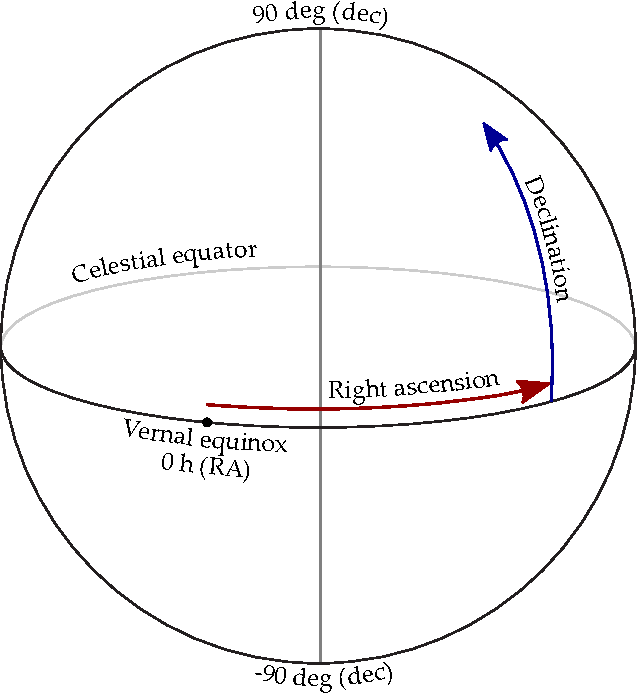
\includegraphics[width=0.5\textwidth]{images/ra-dec}
                \caption{The equatorial coordinate system used in astronomy.}
                \label{fig:equatorial-coordinates}
            \end{figure}

            Astronomy uses the \emph{equatorial coordinate system} to describe
            the positions of objects on the sky. Each position on the sky is
            described by two numbers: the \emph{right ascension} (RA) and the
            \emph{declination} (dec).

            The right ascension of an object is the angle eastward from the
            vernal equinox to the object along the celestial equator. It is
            measured in hours (h), minutes (min), and seconds (s). There are 60
            seconds in 1 minute, 60 minutes in 1 hour, and 1 hour is equal to 15
            degrees. Right ascension ranges between 0h and 24h, where both 0h
            and 24h are located at the vernal equinox. The declination of an
            object is the angle northward from the celestial equator to the
            object. It is measured in degrees (${}^\circ$), arcminutes ($'$),
            and arcseconds ($"$). Declination ranges between $-90^\circ$ and
            $90^\circ$, where $-90^\circ$ is the declination of the south
            celestial pole and $90^\circ$ is the declination of the north
            celestial pole. The right ascension and declination are shown in
            Figure \ref{fig:equatorial-coordinates}. It is important to note
            that while right ascension and declination are both measured in
            minutes and seconds, these are \emph{different} minutes and seconds.
            1 minute (right ascension) is equal to 15 arcminutes (declination).

            Objects are usually given a International Astronomical Union (IAU)
            name based on their coordinates. This name includes the catalogue
            that identified the object, the right ascension, and the
            declination. For example, ATLAS3 J002925.7-440256C is from the third
            release of the ATLAS catalogue, and is located at $00$h $29$m
            $25.7$s $-44^\circ$ $02'$ $56"$.

        \subsection{Wavelength and Frequency}
        \label{sec:wavelength}

            Light is an electromagnetic wave and can thus be characterised by
            its \emph{wavelength} and \emph{frequency} \citep{griffiths99}. The
            wavelength of light is the distance between two neighbouring peaks;
            it is measured in metres (m) and usually denoted $\lambda$. The
            frequency of light is the number of waves that have passed a point
            per second; it is measured in hertz (Hz) and usually denoted $\nu$.
            Wavelength and frequency are related by the formula
            \[
                c = \lambda \nu,
            \]
            where $c$ is the speed of light.

            Humans can see a limited range of wavelengths of light. In this
            range, the wavelength of light corresponds to its colour: Blue light
            has shorter wavelength (and higher frequency) than red light.
            Outside of this range, light still has various different
            ``colours'', but we cannot see them. Different ranges of wavelength
            are assigned different names, such as infrared, x-ray, and radio.

            When objects emit light, the wavelength depends on the process by
            which the light was emitted. For example, thermal radiation is
            emitted by all objects based entirely on the temperature of the
            object, with hotter objects emitting light with shorter wavelengths.
            Another example is synchrotron radiation (Section \ref{sec:agns}),
            which is emitted in radio wavelengths.

            Since telescopes generally only detect brightnesses of objects in
            the sky, and different wavelengths of radiation require different
            mechanisms to detect, telescopes are designed to measure radiation
            only at specific ranges of wavelengths. To gain full scientific
            insight into objects detected in different wavelengths, the objects
            must be cross-identified with each other.

        \subsection{Flux and Magnitude}

            The \emph{flux density} of an object is its energy output per unit
            time per unit area. It is denoted $f$ and is measured in $\text{W
            m}^{-2}$. The flux density is given by
            \[
                f = \frac{1}{A}\frac{\text{d}E}{\text{d}t}
            \]
            where $E$ is the energy received from the object, $t$ is the time,
            and $A$ is the apparent area of the object. We cannot usually
            measure the flux over all frequencies, so flux is observed over a
            specific frequency range $\Delta \nu$. The \emph{spectral flux
            density} is then the limit as the frequency range approaches zero,
            i.e.
            \[
                f_\nu = \frac{1}{A}\frac{\text{d}^2E}{\text{d}\nu\text{d}t}
            \]
            The spectral flux density is measured in janskys (Jy), an
            astronomical unit equal to $10^{-26} \text{ W m}^{-2} \text{
            Hz}^{-1}$ \citep{francis08}.

            The \emph{apparent magnitude}, $m$, of an object is a logarithmic
            measure of its flux seen from Earth, relative to the star Vega
            \citep{francis08}:
            \begin{equation}
                \label{eq:apparent-magnitude}
                m = -2.5 \log_{10} \left(\frac{f}{f_{\text{Vega}}}\right).
            \end{equation}
            $f$ is the flux density of the object and $f_{\text{Vega}}$ is the
            flux density of Vega measured at the same frequency.

            The difference between the magnitudes of two objects, $m_1$ and
            $m_2$, represents the logarithm of the ratio of their flux
            densities:
            \begin{equation}
                \label{eq:magnitude-difference}
                m_2 - m_1 = -2.5 \log_{10} \left(\frac{f_2}{f_1}\right).
            \end{equation}

    \section{Radio Active Galactic Nuclei}
    \label{sec:agns}

        \begin{figure}[!ht]
            \centering
            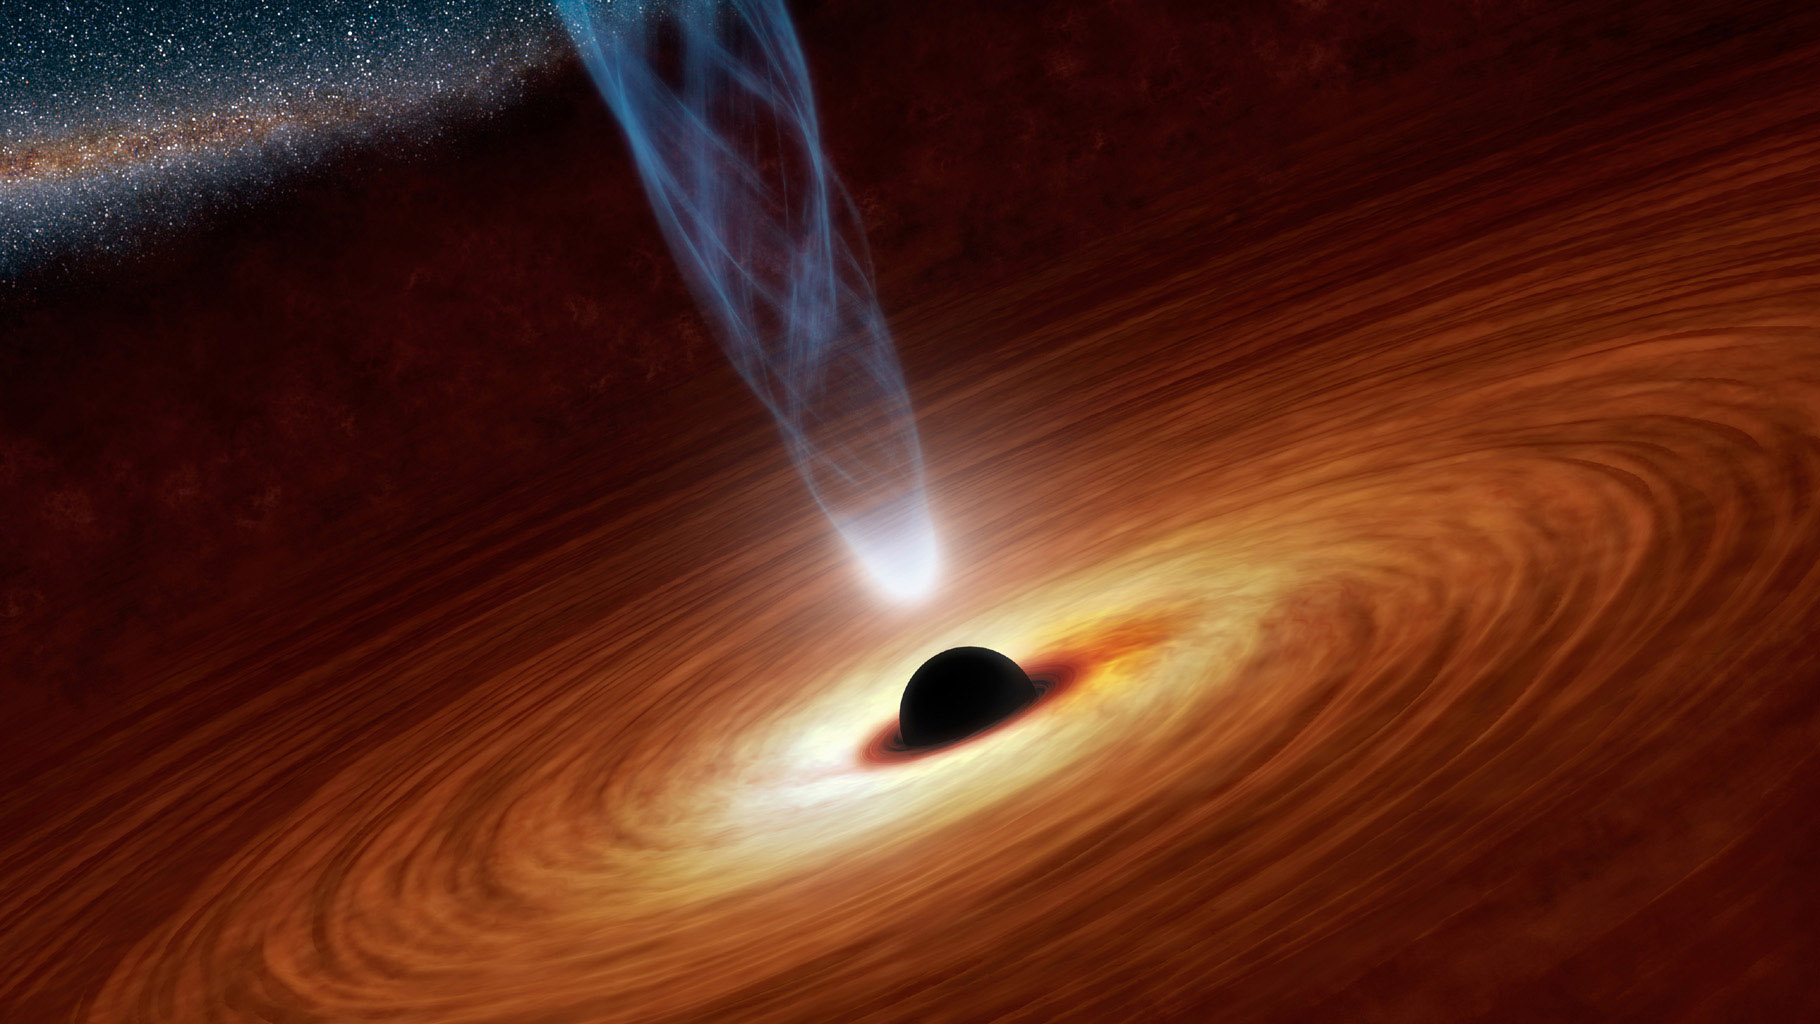
\includegraphics[height=0.2\textheight]
                {images/accretion_disk_artist_impression.jpg}
            \caption{An artist's impression of the accretion disk of an active
                galactic nucleus. \emph{Image: NASA/JPL-Caltech}}
            \label{fig:accretion-disk}
        \end{figure}

        Many galaxies contain a supermassive black hole in their centre
        \citep{richstone98}. These black holes may accrete matter from the
        surrounding galaxy into an \emph{accretion disc} (Figure
        \ref{fig:accretion-disk}). The accretion process emits huge amounts of
        light through different physical processes. These light-emitting black
        holes are called active galactic nuclei (AGNs). AGNs can be extremely
        bright, emitting up to $10^{39}$ J of energy every second --- nearly a
        thousand times more energy than our entire galaxy emits
        \citep{begelman84}. AGNs are found throughout the universe, with the
        closest known AGN being Centaurus A (Figure \ref{fig:centaurus-a}) at a
        distance of around $2.4 \times 10^{20}$ km.

        \begin{figure}
            \centering
            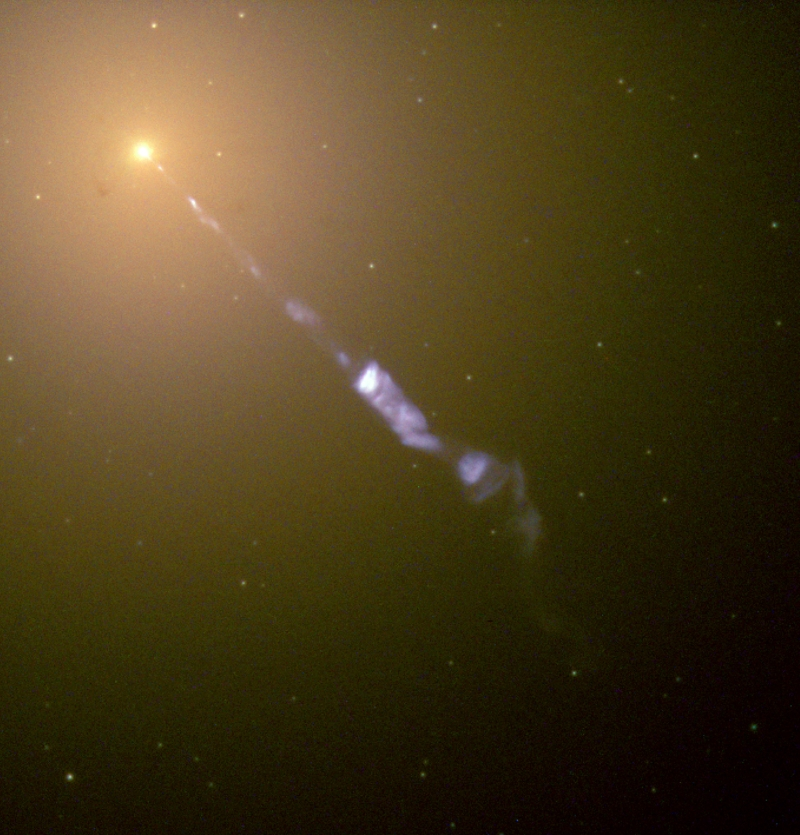
\includegraphics[height=0.3\textheight]{images/M87_jet.jpg}
            \caption{M87, a giant elliptical galaxy with a jet. \emph{Image:
                NASA and The Hubble Heritage Team (STScI/AURA)}}
            \label{fig:m87}
        \end{figure}

        Around 10\% of AGNs produce \emph{jets} from their accretion disk
        \citep{fabian99}. Jets are long, thin streams of matter such as the one
        shown in Figure \ref{fig:m87}. These jets can be very large, with
        ``giant'' AGNs emitting jets nearly $1$ Mpc ($3 \times 10^{19}$ km) in
        length \citep{saripalli05}.

        Electrons in jets produce \emph{synchrotron radiation}. This is a
        form of radiation emitted by charged particles travelling at
        relativistic speeds as they accelerate in a magnetic field
        \citep{sokolov67}. Synchrotron radiation is emitted in radio
        wavelengths, and so AGNs emitting synchrotron radiation are called
        \emph{radio AGNs}. As radio AGNs are the focus of this work, ``AGN''
        will henceforth refer only to radio AGNs unless otherwise specified.

        \begin{figure}
            \centering
            \begin{subfigure}{0.4\textwidth}
                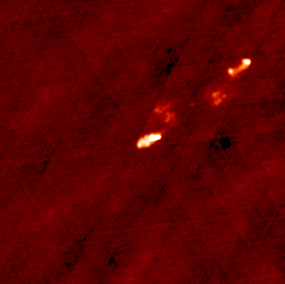
\includegraphics[width=\textwidth]
                    {images/FIRST_093244.58+161050.7.PNG}
                \caption{FIRSTJ093244.5+161050.}
                \label{fig:first-triple}
            \end{subfigure}%
            ~
            \begin{subfigure}{0.4\textwidth}
                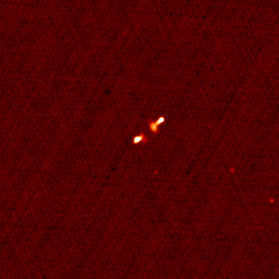
\includegraphics[width=\textwidth]
                    {images/FIRST_130117.5+104121.PNG}
                \caption{FIRSTJ130117.5+104121.}
                \label{fig:first-double}
            \end{subfigure}%
            \caption{Two radio AGNs imaged by the NRAO Very Large Array.}
            \label{fig:first-agn}
        \end{figure}

        We can observe the jets of radio AGNs with radio telescopes, such as in
        Figure \ref{fig:first-agn}. The jets may appear to be separate objects,
        and there may or may not be a radio source in the middle of the AGN
        system. If the system is composed of two separate objects such as in
        Figure \ref{fig:first-double} (one object for each lobe of the jets),
        then it is called a \emph{radio double}; if a central source is also
        visible, then it is called a \emph{radio triple}.

        Since these jets are not point-like sources
        of light, and viewing the jets is the only way to observe radio AGNs,
        common astronomical problems such as cross-identification (Section
        \ref{sec:radio-cross-identification}) can be very difficult, as the true
        location of the AGN is unclear.
        % Most of the radio objects that we have seen in radio surveys conducted
        % so far are these jets \citep{norris11}. Since these jets are the only
        % way to observe radio AGNs, radio AGNs do not appear at all in surveys
        % at other wavelengths.

        % An important part of astronomical surveys is matching objects 

        % To fully understand these objects astronomers need data from more than
        % just radio surveys. Combining observations of objects in multiple
        % wavelengths is therefore a common problem in astronomy, and is called
        % \emph{cross-identification} \citep{fan15}. For point sources of light
        % this can be straightforward --- the coordinates of each source on the
        % sky are well-known and can often be immediately matched throughout
        % surveys --- but as it is the jets of AGNs that emit radio, AGNs are not
        % point sources. We discuss this in detail in Section
        % \ref{sec:radio-cross-identification}.

    \section{Infrared Surveys}
    \label{sec:infrared-surveys}

        A \emph{survey} is an image of the sky made with repeated observations
        in specific wavelengths, aiming to comprehensively cover some large area
        of the sky. In this section we look at WISE and SWIRE, two surveys in
        infrared wavelengths from which we draw data for our experiments.

        \begin{figure}
            \centering
            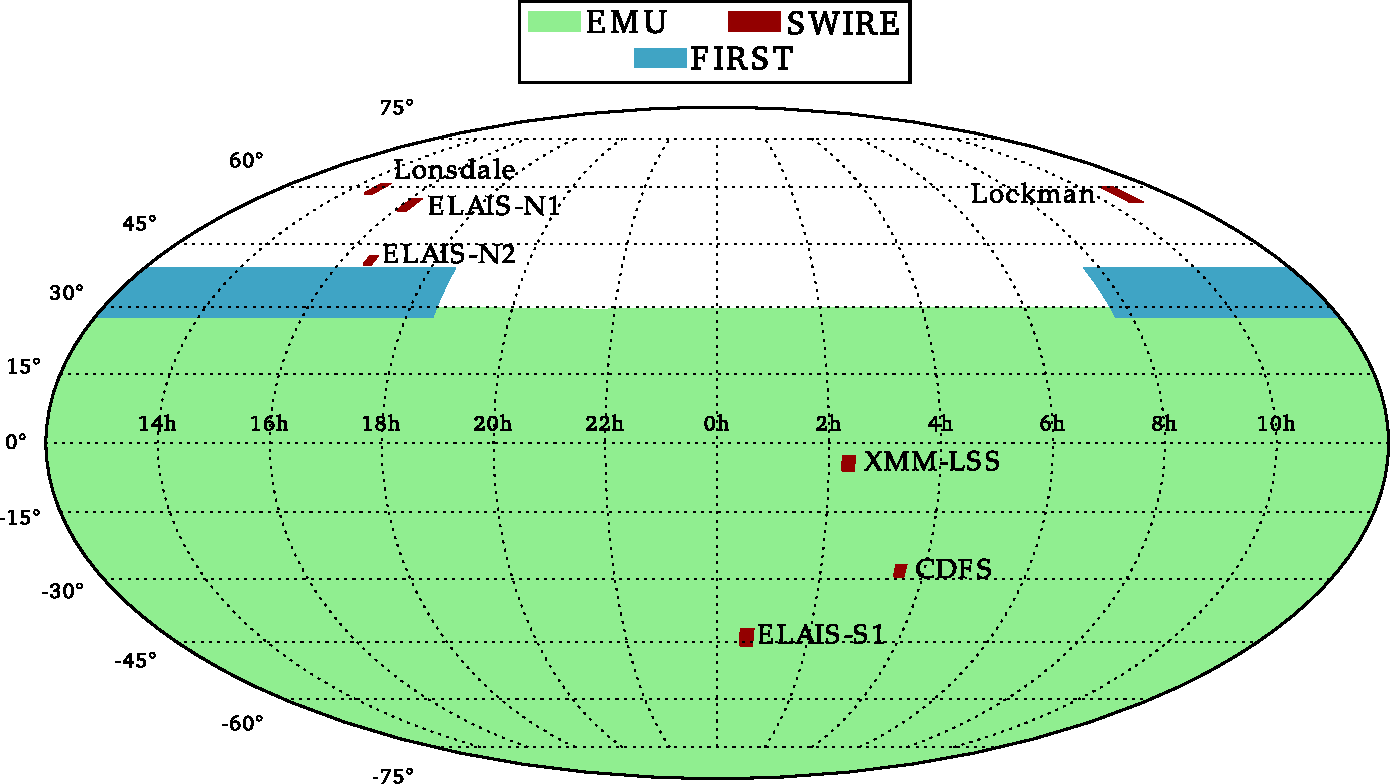
\includegraphics[width=0.8\textwidth]{images/skymap2.pdf}
            \caption{A map of the sky, showing the FIRST and EMU radio surveys,
                and the SWIRE infrared survey. The ATLAS radio survey
                covers both the CDFS and ELAIS-S1 fields. The WISE infrared
                survey covers the entire sky.}
        \end{figure}

        \subsection{WISE: Wide-field Infrared Survey Explorer}
        \label{sec:wise}

            \begin{figure}
                \centering
                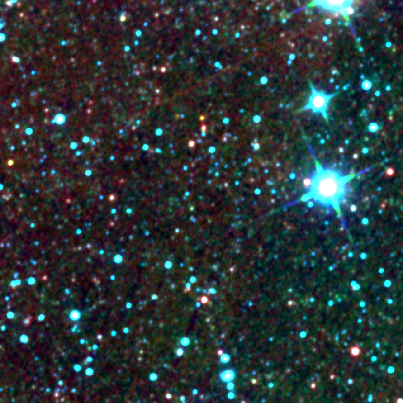
\includegraphics[width=0.5\textwidth]
                    {images/WISE_3h30m05.24s-28d34m46.3s.png}
                \caption{Patch of the WISE multi-wavelength composite image
                    centred on 3h30m05.24s -28d34m46.3s.}
                \label{fig:wise}
            \end{figure}

            The Wide-field Infrared Survey Explorer (WISE) is an orbital
            infrared telescope. In 2009--2010 it was used to survey the entire
            sky in four wavelengths: 3.4 $\mu$m, 4.6 $\mu$m, 12 $\mu$m, and 22
            $\mu$m. These wavelengths are referred to as WISE bands $w1$, $w2$,
            $w3$, and $w4$, respectively. WISE images have resolutions of
            $6''$--$12''$, with sensitivity between $0.08$ and $6$ mJy,
            corresponding to the detection of sources between $16.5$ and $7.9$
            magnitude \citep{wright10}.

            The AllWISE catalogue \citep{cutri13} is the most recent WISE
            catalogue. For each object detected, the catalogue includes the
            magnitudes in each WISE band, as well as a number of other features
            we do not make use of in our methods. We will refer to the
            magnitudes in each band by the names of the bands (i.e. $w1$ --
            $w4$).

            The main goal of WISE was to provide a map of the whole sky in
            infrared wavelengths for many different reasons: infrared
            measurements may be used to detect and classify distant galaxies,
            measurements can be cross-identified to complement other surveys,
            and so on. There are many other scientific goals of WISE; these are
            described in detail by \citet{wright10}.

        \subsection{SWIRE: Spitzer Wide-area Infrared Extragalactic Survey}
        \label{sec:swire}

            \begin{figure}
                \centering
                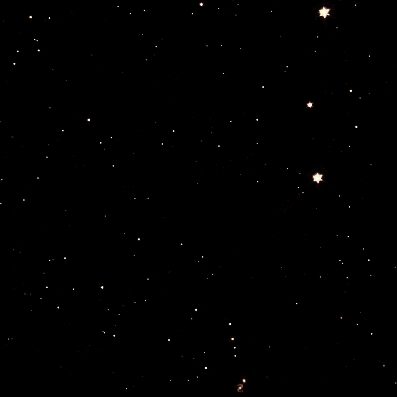
\includegraphics[width=0.5\textwidth]{images/swire_small.jpg}
                \caption{Patch of the SWIRE multi-wavelength composite image
                    centred on 3h30m05.24s -28d34m46.3s. This is the same region
                    of the sky as the WISE image in Figure \ref{fig:wise}.}
            \end{figure}

            The Spitzer Wide-area Infrared Extragalactic Survey (SWIRE) is a
            multi-wavelength infrared survey \citep{lonsdale03}. It observed at
            four wavelengths: 3.6 $\mu$m, 4.5 $\mu$m, 5.8 $\mu$m, and 8.0
            $\mu$m.

            SWIRE surveyed seven fields. These fields --- ELAIS-S1, ELAIS-N1,
            ELAIS-N2, Lockman, CDFS, XMM-LSS, and Lonsdale --- are called the
            \emph{SWIRE fields}, totalling 63.2 square degrees in area. The
            fields contain few nearby objects, meaning that observations in
            these fields are of very old, distant objects. ELAIS-S1 and CDFS are
            in the southern sky; all other fields are in the northern sky.

            While SWIRE covers far less area of the sky than WISE, it does so at
            considerably higher resolution and sensitivity: $1.2''$ and
            $7.3$--$32.5$ $\mu$Jy, respectively \citep{irac-pocket-guide,
            surace05}.

            SWIRE aimed to investigate the evolution of galaxies and AGNs and
            the relationship between galaxies and AGNs \citep{surace05}.

            % In this thesis, we are interested in the Chandra Deep Field South
            % (CDFS), and the European Large Area ISO Survey - South 1 (ELAIS-S1)
            % field. We will use these 

    \section{Radio Surveys}
    \label{sec:radio-surveys}

        In this section we look at the EMU and ATLAS radio surveys. EMU does not
        yet exist, but motivates our work. We will use ATLAS for the experiments
        in later chapters.

        \subsection{EMU: Evolutionary Map of the Universe}
        \label{sec:emu}

            % The largest existing radio survey is currently the NRAO VLA Sky
            % Survey (NVSS) \citep{condon98}, which covers the entire northern sky
            % as far south as $-40^\circ$. However, NVSS has low sensitivity, only
            % detecting objects brighter than $2.5$ mJy. NVSS also has relatively
            % low resolution, only resolving objects to $45''$. The most sensitive
            % existing radio survey is of the Lockman hole \citep{owen08}, which
            % only covered around $0.1$ square degrees of the sky, but detected
            % objects as dim as $0.015$ mJy with an angular resolution of $1.6''$.

            The Evolutionary Map of the Universe (EMU) is an upcoming deep radio
            survey that aims to provide both high sensitivity and wide coverage
            of the radio sky \citep{norris11}. EMU will be sensitive to objects
            to around $0.015$ mJy with an angular resolution of around $10''$,
            and cover the entire southern sky as far north as $30^\circ$. For
            comparison, the largest existing radio survey is currently NVSS
            \citep{condon98} with sensitivity of $2.5$ mJy and a resolution of
            $45''$, which covers a similar area. With the resolution,
            sensitivity, and scale of EMU, astronomers hope to investigate
            galactic evolution, to explore large-scale structure and cosmology
            of the universe, and to find never-before-seen astronomical objects.

            EMU is expected to find huge numbers of radio objects --- while the
            Australia Telescope Large Area Survey [ATLAS] (which has similar
            resolution and sensitivity to EMU) has detected around 4000 radio
            objects, EMU is expected to find \emph{70 million}
            \citep{banfield15}. With such a large number of detected objects,
            analysis of the data from EMU will be considerably more difficult
            than analysis of existing surveys. This analysis will be impossible
            by hand, and will therefore require algorithms to process the data.
            With so many new objects it is likely that many objects will not fit
            existing models, meaning that model-based approaches to data
            processing may be ineffective. \citet{norris11} estimated that 10\%
            of the newly-found objects will be too complicated for current
            automated algorithms \citep{banfield15}. It is this problem that
            motivates the development of new, machine-learned algorithms for
            processing astronomical data at these large scales. While the EMU
            survey data is not yet released, development of such algorithms can
            begin by looking at other datasets with similar sensitivity and
            resolution, such as ATLAS (Section \ref{sec:atlas}).

            The radio objects found by EMU will eventually be cross-identified
            with the infrared objects found by WISE (Section \ref{sec:wise}). As
            such, any algorithms that we develop must work with WISE data.

        \subsection{ATLAS: The Australia Telescope Large Area Survey}
        \label{sec:atlas}

            \begin{figure}
                \centering
                \includegraphics[width=0.8\linewidth,]{images/CDFS_bitmap}
                \caption{ATLAS observations of CDFS.
                    Reproduced from \citet{franzen15}.}.
                \label{fig:cdfs}
            \end{figure}

            The Australia Telescope Large Area Survey (ATLAS) is a high
            sensitivity radio survey which aims to help understand the evolution
            of early galaxies \citep{norris06}. The Australia Telescope Compact
            Array was used to image two small areas of the sky: CDFS and
            ELAIS-S1. These fields in particular were chosen because they are
            the two fields imaged in SWIRE (Section \ref{sec:swire}) visible from
            the southern hemisphere. SWIRE produced high-resolution infrared
            images of its fields, allowing all objects detected in the ATLAS
            radio images to be cross-identified with their infrared
            counterparts.

            ATLAS is considered a pilot survey for EMU. EMU and ATLAS image the
            same wavelengths with similar resolution and sensitivity, so tools
            and methods developed to process and interpret ATLAS data are
            expected to work well on the data produced by EMU.

            ATLAS provides both a catalogue of detected radio objects and a
            radio image of the CDFS and ELAIS-S1 fields. The CDFS image covers a
            total area of 3.7 square degrees and the ELAIS-S1 image covers a
            total area of 2.7 square degrees. The CDFS image is shown in Figure
            \ref{fig:cdfs}. The catalogue is a list of all objects detected in
            the images with a peak or integrated flux more than 5 times the
            background noise levels. For each object, the catalogue lists
            \begin{itemize}
                \setlength\itemsep{0 pt}
                \item an survey identifier,
                \item an IAU name,
                \item a position on the sky of the peak flux,
                \item a peak flux density,
                \item an integrated flux density,
                \item an angular size,
                \item whether the object is extended or compact, and
                \item a spectral index,
            \end{itemize}
            as well as uncertainties associated with each measurement
            \citep{franzen15}.

            The ATLAS survey of the CDFS field is the focus of our experiments
            for three main reasons. It contains around 2400 objects, providing
            enough training data for machine learning methods, but still
            remaining a manageable size for our resource-limited tests. As a
            pilot survey for EMU, we expect methods developed on ATLAS to also
            work on EMU. Finally, we have three sets of cross-identifications
            for ATLAS-CDFS (see Sections
            \ref{sec:radio-cross-identification} and
            \ref{sec:radio-galaxy-zoo}), allowing us to check the performance of
            methods we develop.

    \section{Radio Cross-identification}
    \label{sec:radio-cross-identification}

        % \subsection{Motivation}
        % \label{sec:cross-identification-motivation}

        Observations of astronomical objects in different wavelengths give us
        information on different physical properties of the objects. We can only
        make use of this information, however, if we can match observations of
        the same object in different surveys. This is called
        \emph{cross-identification}.

        The specific cross-identification task we focus on in this thesis is
        that of cross-identifying a radio object with the associated infrared
        object. Most often in current radio surveys, a radio object will be a
        jet from an AGN \citep{norris11}. In this case, we refer to the infrared
        counterpart as the \emph{host galaxy} of the AGN. We will assume that
        all radio objects are AGNs. The main goal of cross-identifying AGNs is
        to better understand the relationship between AGNs and star-forming
        activity in their host galaxies \citep{norris06}.

        Sometimes, cross-identification is easy: We may have point-like sources
        of light, allowing us to simply overlay two surveys and identify
        overlapping objects. In the case of cross-identifying radio AGNs,
        though, we do not have point-like sources of light, and
        cross-identification can be very difficult. AGN jets may be arbitrarily
        large and complex, and often show up as multiple disconnected radio
        objects. As such, past attempts to cross-identify radio objects have
        required human insight
        \citep{norris06,fan15}.

        In this section, we look at two different ways astronomers have
        cross-identified radio objects in the CDFS field of the ATLAS survey. We
        will make use of the resulting catalogues for testing our
        cross-identification methods in Chapters \ref{cha:cross-identification}
        and \ref{cha:active-learning}.

        % While we cannot observe the black holes of AGNs directly, we can observe
        % the radio emissions from their jets. These could then be matched to the
        % galaxies hosting the black holes, allowing us to learn more about the
        % galaxy, the black hole, and the surrounding environment. These host
        % galaxies are not visible in radio wavelengths,

        \subsection{Norris et al. Catalogue}
        \label{sec:norris}

            Along with a catalogue of radio objects found in the CDFS field by
            the ATLAS survey, \citet{norris06} produced a catalogue of
            cross-identifications of these radio objects. The catalogue lists
            ATLAS objects and their corresponding SWIRE objects.

            The cross-identification process was semi-automated.
            \citeauthor{norris06} first matched each ATLAS object to the nearest
            SWIRE object. After this step, around half of the radio objects were
            matched to a SWIRE object within $1''$, and $79\%$ were matched to a
            SWIRE object within $3''$. Radio objects greater than $3''$ away
            from a SWIRE object were then cross-identified manually; radio
            doubles and radio triples were matched to the SWIRE object nearest
            their centre.

            Additionally, \citeauthor{norris06} found between 8 and 22 radio
            objects with no identifiable host galaxy in the infrared. These are
            called ``infrared-faint'' radio objects.

            \citeauthor{norris06} estimated the probability of false
            cross-identifications by displacing all radio objects by $1'$ and
            repeating the cross-identification process. From the results of this
            test, they estimated that $9.02\%$ of the cross-identifications are
            false.

            We consider these cross-identifications \emph{expert}
            cross-identifications, i.e., they are the best possible
            cross-identifications available for radio objects in the CDFS field.
            Throughout this thesis, we will use these as an approximation to the
            unobservable groundtruth cross-identifications.

        \subsection{Fan et al. Catalogue}
        \label{sec:fan}

            \citet{fan15} developed an automated cross-identification algorithm
            that fits astronomical models of AGNs to the radio sky.

            The algorithm examines each infrared object in turn. Under the
            assumption that the infrared object is a host galaxy, it then
            searches in a $2'$ radius for potential radio components of AGN
            jets. The radio components with highest likelihood according to a
            Bayesian model are selected using a greedy algorithm.

            This method has some clear limitations --- it is model-based, and
            thus may fail for unexpected radio objects like those we might find
            in EMU, and it is not able to cross-identify infrared-faint radio
            objects. Nevertheless, it performs very well when applied to the
            ATLAS-CDFS field, making 564 cross-identifications identically to
            \citeauthor{norris06}, missing 31 cross-identifications that
            \citeauthor{norris06} reported, and cross-identifying an additional
            62 radio objects.

            We consider the \citeauthor{fan15} cross-identifications of
            ATLAS-CDFS as an alternative source of expert cross-identifications,
            due to the high (but not total) agreement with the
            \citeauthor{norris06} catalogue.

    \section{Radio Galaxy Zoo}
    \label{sec:radio-galaxy-zoo}

        \begin{figure}
            \centering
            \begin{subfigure}[t]{0.3\textwidth}
                \centering
                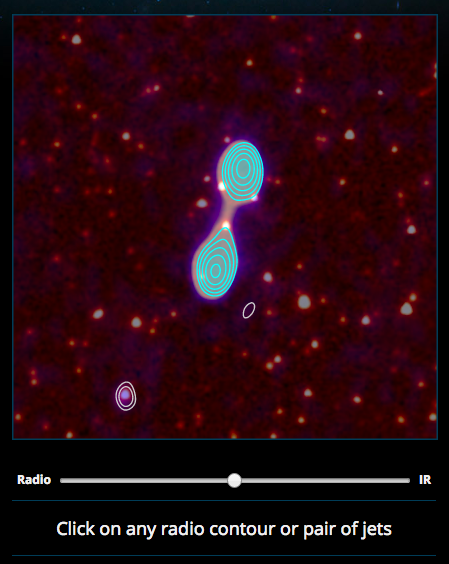
\includegraphics[height=2in]{images/rgz_radio.png}
                % These empty captions give us something to reference later.
                \caption{}
                \label{fig:rgz-interface-a}
            \end{subfigure}%
            ~
            \begin{subfigure}[t]{0.3\textwidth}
                \centering
                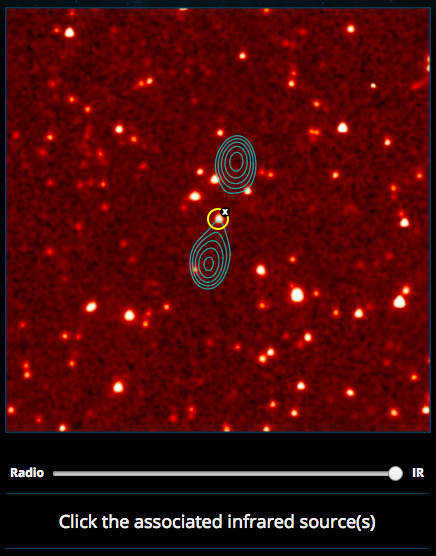
\includegraphics[height=2in]{images/rgz_ir.png}
                \caption{}
                \label{fig:rgz-interface-b}
            \end{subfigure}%
            ~
            \begin{subfigure}[t]{0.3\textwidth}
                \centering
                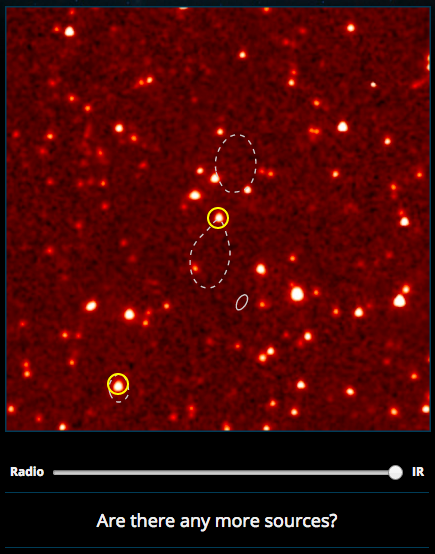
\includegraphics[height=2in]{images/rgz_done.png}
                \caption{}
                \label{fig:rgz-interface-c}
            \end{subfigure}
            \caption{Radio Galaxy Zoo volunteer workflow.\\
                \protect\makebox[1.5cm][r]{\ref{fig:rgz-interface-a}}
                    Volunteers are first asked to identify associated radio
                    objects.\\
                \protect\makebox[1.5cm][r]{\ref{fig:rgz-interface-b}}
                    Volunteers then cross-identify the radio objects with the
                    corresponding host galaxy.\\
                \protect\makebox[1.5cm][r]{\ref{fig:rgz-interface-c}}
                    This is repeated for all radio objects in the image.}
            \label{fig:rgz-interface}
        \end{figure}

    The \citeauthor{norris06} catalogue is highly accurate, but manual expert
    cross-identification of radio surveys is impractical for large surveys. The
    CDFS field examined by \citeauthor{norris06} only contains around 2400 radio
    objects, which is small even compared to existing surveys (e.g. Faint Images
    of the Radio Sky at Twenty-Centimeters (FIRST) \citep{becker95} found
    946~000 radio sources). Automated algorithms such as \citeauthor{fan15}
    scale better, but most such algorithms are still in their infancy
    \citeauthor{norris16} and many are model-based, potentially missing many
    sources that do not fit the models. The Radio Galaxy Zoo project
    \citep{banfield15} provides a different approach: Allow many non-expert
    volunteers to manually cross-identify radio sources with their infrared host
    galaxies.

    Radio Galaxy Zoo\footnote{\url{http://radio.galaxyzoo.org/}} is a website
    where volunteers are presented with a radio image from ATLAS or FIRST and a
    corresponding infrared image from SWIRE or WISE, and are tasked with
    matching the radio source with its host galaxy, as well as identifying which
    radio objects are associated with the same host galaxy (e.g., two radio
    objects may represent two jets of one AGN). To help reduce noise in these
    matches, each compact radio object is shown to 5 volunteers, and each
    complex radio object is shown to 20 volunteers. While both the
    cross-identification task and the radio object association task are
    astronomically interesting, we focus only on the cross-identification task
    for this thesis. An example of the workflow presented to volunteers is shown
    in Figure \ref{fig:rgz-interface}.

    Since its launch in December 2013, the Radio Galaxy Zoo project has labelled
    over 100~000 radio objects. One particularly notable result is the discovery
    of one of the largest known wide-angled tail AGNs by two volunteers, which
    would be impossible to detect in current automated algorithms
    \citep{banfield16}.

    The Radio Galaxy Zoo dataset contains around 177~000 images from FIRST, and
    2400 images of the CDFS field from ATLAS. The ATLAS images of the ELAIS-S1
    field are not included, and may be used as a testing set for
    cross-identification algorithms trained on the Radio Galaxy Zoo in the
    future. Each image is a 2 arcminute-wide square.

    The cross-identifications are stored in a MongoDB database as a collection
    of associated radio objects and the corresponding pixel locations of the
    volunteers' clicks, as well as the right ascension and declination of the
    radio object. The radio and infrared image patches associated with each
    radio object are also included alongside the database. For detailed analysis
    of these labels, see \citet{atlas-ml}.

    In Chapter \ref{cha:cross-identification}, we will train machine learning
    algorithms to perform the cross-identification task trained on ATLAS-CDFS
    labels from the Radio Galaxy Zoo.

%     Radio Galaxy Zoo volunteers are first asked to select combinations of
%     radio objects that correspond to one radio source, and are then asked to
%     select the location of the corresponding host galaxy \citep{banfield15}.
%     Each radio subject is labelled by multiple volunteers. These labels are
%     then collated as follows. First, the most common combination of radio
%     objects is selected, and all labels that have a different combination are
%     discarded. This radio combination is called the consensus radio
%     combination. Then, the density of host location labels is estimated using
%     Gaussian kernel density estimation (KDE), and the highest density location
%     is selected. This is called the consensus host location. The consensus
%     host location is then matched to the nearest infrared object.

%     An alternative way to find the consensus host location is by using a
%     clustering algorithm such as $k$-means. Host locations are clustered and
%     the cluster containing the most locations is taken to represent the
%     consensus; the consensus location is then the mean of the cluster. This is
%     faster and more robust than using KDE, but requires $k$ to be known. $k$
%     can be estimated using an algorithm such as PG-means \citep{hamerly07} or
%     by choosing $k$ to minimise some information criterion
%     \todo{cite:sklearn}. The consensus labels for the data associated with
%     this thesis were found in this way, fitting a Gaussian mixture model to
%     the host locations with the number of Gaussians chosen to minimise the
%     Bayesian information criterion.

%     Repeated volunteer labelling helps to reduce noise in the labels. This is
%     necessary as the volunteers are not experts, and may incorrectly label the
%     subject. The hope is that the majority of volunteers will correctly label
%     subjects, which seems to be the case for radio subjects where more than
%     75\% of volunteers agree \citep{banfield15}. The number of times a radio
%     subject is shown to different volunteers is called the redundancy. The
%     redundancy is 5 if the subject is a compact source, and 20 for all other
%     sources. These numbers were chosen based on the redundancy levels of the
%     original Galaxy Zoo project [Banfield, personal communication] \todo{Is
%     this how to cite personal communication? Alternatively, is this written
%     down somewhere?}. Since labels with radio combinations that disagree with
%     the consensus are discarded, the redundancy is usually lower in practice
%     when finding the host location. This can lead to very low redundancy input
%     to KDE, causing KDE to fail. This failure can usually be caught, but the
%     existing solution in this case is to take the mean of all host locations.
%     This is not the consensus host location in general. Another effect is that
%     since more complex sources have higher levels of disagreement in the radio
%     combination stage, more complex sources have more discarded volunteer
%     labels, and thus lower redundancy --- so more complex sources have more
%     noise in their labels.
